\documentclass[12pt]{Homework}

% Changed from \usepackage{prelude}
\usepackage{preamble}
\usepackage{amssymb}
\usepackage{enumitem}
\usepackage{mathrsfs}
\def\upint{\mathchoice%
    {\mkern13mu\overline{\vphantom{\intop}\mkern7mu}\mkern-20mu}%
    {\mkern7mu\overline{\vphantom{\intop}\mkern7mu}\mkern-14mu}%
    {\mkern7mu\overline{\vphantom{\intop}\mkern7mu}\mkern-14mu}%
    {\mkern7mu\overline{\vphantom{\intop}\mkern7mu}\mkern-14mu}%
  \int}
\def\lowint{\mkern3mu\underline{\vphantom{\intop}\mkern7mu}\mkern-10mu\int}
\usepackage[mathscr]{euscript}
\usepackage{comment}
\usepackage{MnSymbol}
\usepackage{tikz,float}
\usepackage{tikz-cd}
\usepackage{graphicx}
\usepackage{mathtools}
\usepackage{bbding}
\renewcommand\qedsymbol{\Peace}
\newcommand\placeqed{\nobreak\enspace\Peace}
\usepackage{caption, threeparttable}
\usepackage{halloweenmath}
\newcommand{\contradiction}{\null\hfill\large{$\mathghost$}\normalsize}
\newcommand{\im}{\mathscr{I}\text{m}}
\newcommand{\re}{\mathscr{R}\text{e}}
\newcommand{\res}{\text{Res}}

\name{Kayla Orlinsky}
\course{Complex Analysis Exam}
\term{Fall 2016}
\hwnum{Fall 2016}

\begin{document}

\begin{problem} $\,$
Let $A=\{z\in\mathbb{C}:r<|z|<R\}$ for some $0<r<R<\infty.$ Prove that $f(z)=1/z$ cannot be uniformly approximated in $A$ by complex polynomials.
\end{problem}


\begin{solution}$\,$
Let $\{p_n(z)\}$ be a sequence of polynomials converging uniformly to $f$ on $A$.

Let $\varepsilon>0$ and $N$ such that $|f(z)-p_n(z)|<\varepsilon$ for all $n\ge N$ and all $z\in A$.

Then $$|p_n(z)|-|f(z)|\le|f(z)-p_n(z)|<\varepsilon$$ and so $$|zp_n(z)|<\varepsilon|z|+1.$$

Let $q_n(z)=zp_n(z)$. Then $q_n$ is entire so on $\{|z|\le M\}$ $$|q_n(z)|\le \varepsilon M+1.$$ Therefore, by the Cauchy Estimate, on $\{|z|\le M\}$, $$|q_n^{(2)}(z)|\le\frac{2!(1+\varepsilon M)}{M^2}\to0\qquad M\to\infty.$$

Therefore, there exists $a,b\in\mathbb{C}$ so $q_n(z)=az+b=zp_n(z)$ and so $$p_n(z)=a+\frac{b}{z}$$ which is clearly a contradiction since $p_n$ is a polynomial.

Thus, no such sequence can exist.
\end{solution}
\newpage



\begin{problem} $\,$
Let $D=\mathbb{C}\backslash[-1,1]$. Prove that $f(z)=z^2-1$, for $z\in D$, has an analytic square root but does not have an analytic logarithm. 
\end{problem}

\begin{solution}$\,$
This question relies on two key facts

\begin{itemize}[leftmargin=2.5cm]
    \item $f$ is an $n^{th}$ root if and only if $$\frac{1}{2\pi i}\int_\gamma\frac{f'(z)}{f(z)}dz\quad\in n\mathbb{Z}$$
    \item $f$ has an analytic logarithm if and only if $f$ has an analytic $n^{th}$ root for every $n$
\end{itemize}

Since these facts are not immediately obvious, they will be proved here.

\begin{claim} Let $f$ have no zeros in an open (\textit{NOT} necessarily simply connected) region $\Omega$, then $f$ has an $n^{th}$ root if and only if $$\frac{1}{2\pi i}\int_{\gamma}\frac{f'(z)}{f(z)}dz\quad\in n\mathbb{Z}$$ for all closed curves $\gamma\subset\Omega$.
\begin{proof} \boxed{\implies} If $f$ has an $n^{th}$ root, then there exists an analytic $g(z)$ in $\Omega$ such that $f(z)=g^n(z)$.

Thus, for all $\gamma\subset\Omega$ closed, \begin{align*}
    \frac{1}{2\pi i}\int_\gamma\frac{f'(z)}{f(z)}dz&=\frac{1}{2\pi i}\int_\gamma\frac{ng^{n-1}(z)g'(z)}{g^n(z)}dz\\
    &=n\left[\frac{1}{2\pi i}\int_\gamma\frac{g'(z)}{g(z)}dz\right]\\
    &=n(\text{number of zeros of }g\text{ in }\gamma)\\
    &\in n\mathbb{Z}
\end{align*}

\boxed{\impliedby} Let $$\frac{1}{2\pi i}\int_{\gamma}\frac{f'(z)}{f(z)}dz\quad\in n\mathbb{Z}$$ for all closed curves $\gamma\subset\Omega$.

Now, fix some $z_0\in\Omega$ and let $\gamma_z$ be some curve in $\Omega$ from $z_0$ to some $z\in\Omega$.

Given $\gamma_z$ and $\Tilde{\gamma}_z$ two different paths, $\Gamma=\gamma_z\Tilde{\gamma}_z^{-1}$ is a closed path and since $$\frac{1}{n}\int_\Gamma\frac{f'(\xi)}{f(\xi)}d\xi\quad\in 2\pi i\mathbb{Z}$$ we have that $\displaystyle \frac{1}{n}\int_{\gamma_z}\frac{f'(\xi)}{f(\xi)}d\xi$ differs by choice of path by integer multiples of $2\pi i.$

Let $$h(z)=e^{\frac{1}{n}\int_{\gamma_z}\frac{f'(\xi)}{f(\xi)}d\xi}.$$ Then $h$ is independent of choice of $\gamma_z$ and so is well defined.

Finally, since $f$ has no zeros in $\Omega$, then $\frac{f'}{f}$ is analytic in $\Omega$ and so $h'(z)$ exists and $$h'(z)=e^{\frac{1}{n}\int_{\gamma_z}\frac{f'(\xi)}{f(\xi)}d\xi}\frac{f'(z)}{nf(z)}=h(z)\frac{f'(z)}{nf(z)}.$$

\begin{align*}
    \frac{d}{dz}\frac{f(z)}{h^n(z)}&=\frac{f'(z)h^n(z)-nf(z)h^{n-1}(z)h'(z)}{h^{2n}(z)}\\
    &=\frac{f'(z)h^n(z)-nf(z)h^{n-1}(z)h(z)\frac{f'(z)}{nf(z)}}{h^{2n}(z)}\\
    &=\frac{f'(z)h^n(z)-h^n(z)f'(z)}{h^{2n}(z)}\\
    &=0
\end{align*}

Therefore, $\frac{f(z)}{h^n(z)}=c$ some constant and so $f(z)=ch^n(z)=(c^{1/n}h(z))^n$. 

Finally, then $f$ must have an $n^{th}$ root.
\end{proof}
\end{claim}

Now, $$\frac{f'(z)}{f(z)}=\frac{2z}{z^2-1}$$ which has poles at $-1,1\notin D$. Therefore, any closed curve $\gamma\subset D$ either dodges the line segment $[-1,1]$ and so cannot contain either of the two poles, or it wraps around the line segment $[-1,1]$ in which case, it must contain both poles.

Namely, $$\frac{1}{2\pi i}\int_\gamma\frac{f'(z)}{f(z)}dz\in2\mathbb{Z}$$ for all closed curves $\gamma\subset D$.

Thus, by \textbf{Claim 1} a square root of $f$ exists.

Finally, we note that $f$ has an analytic logarithm if and only if $f$ has an analytic $n^{th}$ root for all $n$.

\begin{claim} If $f$ has no zeros in $\Omega$, then $f$ has an analytic logarithm if and only if $f$ has an analytic $n^{th}$ root for all $n$.
\begin{proof} \boxed{\implies} If $f$ has an analytic logarithm, then there exists an analytic $g(z)$ such that $f(z)=e^{g(z)}.$

Thus, for all closed curves $\gamma$, $$\frac{1}{2\pi i}\int_\gamma\frac{f'(z)}{f(z)}dz=\frac{1}{2\pi i}\int_\gamma\frac{e^{g(z)}g'(z)}{e^{g(z)}}dz=\frac{1}{2\pi i}\int_\gamma g'(z)dz=0$$ since $g'$ is also analytic.

Since $0\in n\mathbb{Z}$ for all $n$, by \textbf{Claim 1}, $f$ has an $n^{th}$ root for all $n$.

\boxed{\impliedby} If $f$ has an $n^{th}$ root for all $n$, then $$\frac{1}{2\pi i}\int_\gamma\frac{f'(z)}{f(z)}dz=0$$ for all $\gamma$ closed in the domain.

Namely, $$g(z)=\frac{1}{n}\int_{z_0}^z\frac{f'(z)}{f(z)}dz$$ is an analytic function and well defined for all $z$ and all fixed $z_0$.

Therefore, using the same idea as \textbf{Claim 1}, we get that $f=e^{g(z)}$ where $g$ is analytic and so $f$ has an analytic logarithm in $\Omega.$
\end{proof}
\end{claim}

Therefore, by \textbf{Claim 2}, $f$ cannot have an analytic logarithm, since $\gamma=|z|=2$ gives $$\frac{1}{2\pi i}\int_{|z|=2}\frac{f'(z)}{f(z)}dz=\frac{1}{2\pi i}\int_{|z|=2}\frac{2z}{z^2-1}dz=\res_{z=1}\frac{2z}{z^2-1}+\res_{z=-1}\frac{2z}{z^2-1}=\frac{2}{1+1}+\frac{-2}{-1-1}=2\not=0.$$

\begin{framed}
Note that to actually determine the value of $\displaystyle \int_\gamma\frac{f'}{f}dz$, we can view the integral in $\mathbb{C}$ and apply the argument principle or residue theorem there. 

Since the integral exists in $D$, the two values must be the same.
\end{framed}
\end{solution}
\newpage




\begin{problem} $\,$
Evaluate $$\int_0^\infty\frac{\log x}{1+x^2}dx$$
\end{problem}


\begin{solution}$\,$
We will use ``Ol' Faithful'' the contour around the upper half plane avoiding the origin since every branch cut of $\log x$ intersects $0$.

Then we take any branch which does not intersect the upper half plane (including the real line).
\begin{center}
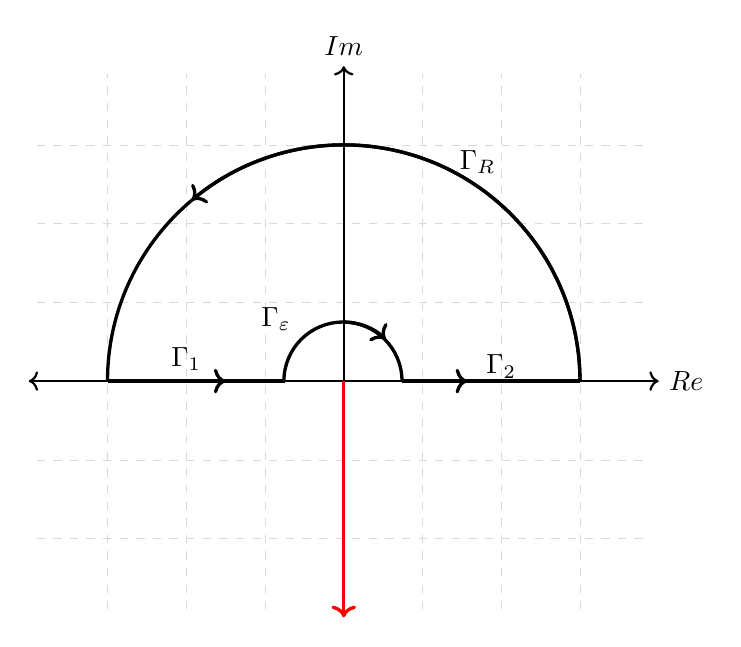
\begin{tikzpicture}
\draw[help lines, color=gray!30, dashed] (-3.9,-2.9) grid (3.9,3.9);
\draw[->,very thick] (3,0) arc (0:130:3cm);
\draw[very thick] (3,0) arc (0:180:3cm) node[above,yshift=2.5cm,xshift=4.7cm]{$\Gamma_R$};
\draw[->,very thick] (0,0.75) arc (90:45:0.75cm);
\draw[very thick] (0.74,0) arc (0:180:0.75cm) node[above,yshift=0.5cm,xshift=-0.1cm]{$\Gamma_\varepsilon$};
\draw[->,very thick] (0.74,0) -- (1.57,0);
\draw[very thick] (0.75,0) -- (3,0) node[above,yshift=-0.1cm,xshift=-1cm]{$\Gamma_2$};
\draw[->,very thick] (-3,0) -- (-1.5,0);
\draw[very thick] (-0.74,0) -- (-3,0) node[above,yshift=0cm,xshift=1cm]{$\Gamma_1$};
\draw[<->, thick] (-4,0)--(4,0) node[right]{$Re$};
\draw[->, thick] (0,0)--(0,4) node[above]{$Im$};
\draw[->,very thick,red] (0,0) -- (0,-3);
\end{tikzpicture}
\end{center}

Let \begin{align*}
    I_1&=\int_{\Gamma_1}\frac{\log z}{z^2+1}dz\\
    I_2&=\int_{\Gamma_2}\frac{\log z}{z^2+1}dz\\
    I_\varepsilon&=\int_{\Gamma_\varepsilon}\frac{\log z}{z^2+1}dz\\
    I_R&=\int_{\Gamma_R}\frac{\log z}{z^2+1}dz
\end{align*}

Now, \begin{align*}
    I_1&=\int_{\Gamma_1}\frac{\log z}{z^2+1}dz\\
    &=\int_{-R}^{-\varepsilon}\frac{\log x}{x^2+1}dx\\
    &=\int_R^\varepsilon\frac{-\log(-x)}{x^2+1}dx\\
    &=\int_\varepsilon^R\frac{\log x+\pi i}{x^2+1}dx\\
    &=I_2+\pi i\tan^{-1}(x)\big|_\varepsilon^R\\
    &=I_2+\pi i(\tan^{-1}(R)-\tan^{-1}(\varepsilon))
\end{align*}

\begin{align*}
    |I_R|&=\left|\int_{\Gamma_R}\frac{\log z}{z^2+1}dz\right|\\
    &\le\int_{\Gamma_R}\frac{|\log z|}{|z^2+1|}d|z|\\
    &\le\int_{\Gamma_R}\frac{|\log z|}{|z|^2-1}d|z|\\
    &=\int_0^\pi\frac{R|\log(Re^{i\theta})|}{R^2-1}d\theta\\
    &=\int_0^\pi\frac{R|\log(R)+i\theta|}{R^2-1}d\theta\\
    &\le\int_0^\pi\frac{R\log(R)+R\pi}{R^2-1}d\theta\\
    &=\pi\frac{R(\log R+\pi)}{R^2-1}\to0\qquad R\to\infty
\end{align*} since $$\lim_{R\to\infty}\frac{R\log R}{R^2-1}=\lim_{R\to\infty}\frac{\log R+1}{2R}\lim_{R\to\infty}\frac{1}{R}=0$$ by L'Hopital's Rule.

Similarly, \begin{align*}
    |I_\varepsilon|&=\left|\int_{\Gamma_\varepsilon}\frac{\log z}{z^2+1}dz\right|\\
    &\le\int_{\Gamma_\varepsilon}\frac{|\log z|}{1-|z|^2}d|z|\\
    &=\int_0^\pi\frac{\varepsilon|\log(\varepsilon e^{i\theta})|}{\varepsilon^2-1}d\theta\\
    &\le\int_0^\pi\frac{\varepsilon\log(\varepsilon)+\varepsilon\pi}{\varepsilon^2-1}d\theta\\
    &=\pi\frac{\varepsilon(\log \varepsilon+\pi)}{\varepsilon^2-1}\to0\qquad \varepsilon\to0
\end{align*} since $$\lim_{\varepsilon\to0}\varepsilon\log\varepsilon=\lim_{\varepsilon\to0}\frac{\log\varepsilon}{\frac{1}{\varepsilon}}=\lim_{\varepsilon\to0}\frac{\frac{1}{\varepsilon}}{-\frac{1}{\varepsilon^2}}=\lim_{\varepsilon\to0}-\varepsilon=0$$ by L'Hopital's Rule.

Finally, by the Residue Theorem, \begin{align*}
    2\pi i\res_{z=i}\frac{\log z}{z^2+1}&=2\pi i\frac{\log(i)}{i+i}\\
    &=\pi\left(\log|i|+i\frac{\pi}{2}\right)\\
    &=i\frac{\pi^2}{2}\\
    &=\lim_{R\to\infty}\lim_{\varepsilon\to0}(I_1+I_2+I_R+I_\varepsilon)\\
    &=2\int_0^\infty\frac{\log x}{1+x^2}dx+\pi i\left(\frac{\pi}{2}\right)\\
    \implies \int_0^\infty\frac{\log x}{1+x^2}dx&=0
\end{align*}

Note that this is consistent with what we found in \textbf{Fall 2013: Problem 1}.
\end{solution}
\newpage





\begin{problem} $\,$
Show that the range of a nonconstant entire function is dense in $\mathbb{C}$.
\end{problem}


\begin{solution}$\,$
Let $f$ be nonconstant and entire. Assume that $f(\mathbb{C})$ is not dense in $\mathbb{C}$.

Then there exists some $z_0\in\mathbb{C}$ and some $\rho>0$ such that $f(\mathbb{C})\cap B_\rho(z_0)=\varnothing$.

Namely, $$|f(z)-z_0|\ge\rho$$ for all $z\in\mathbb{C}$.

However, then we can let $g(z)=\frac{1}{f(z)-z_0}$. Then $g$ is clearly entire but $$|g(z)|=\frac{1}{|f(z)-z_0|}\le\frac{1}{\rho}$$ and so $g$ is bounded on $\mathbb{C}$, so by Louiville's $g$ is constant.

However, then $f$ is constant which is a contradiction.

Thus, if $f$ is non-constant then it is dense in $\mathbb{C}$.

\end{solution}


\end{document}
 